%%%%%%%%%%%%%%%%%%%%%%%%%%%%%%%%%%%%%%%%%%%%%%%%%%%%%%%%%%%%%%%%%%%%%%%%%%%%%%%%
%2345678901234567890123456789012345678901234567890123456789012345678901234567890
%        1         2         3         4         5         6         7         8

\documentclass[letterpaper, 10 pt, conference]{ieeeconf}  % Comment this line out if you need a4paper

%\documentclass[a4paper, 10pt, conference]{ieeeconf}      % Use this line for a4 paper

\IEEEoverridecommandlockouts                              % This command is only needed if 
                                                          % you want to use the \thanks command

\overrideIEEEmargins                                      % Needed to meet printer requirements.
\pdfminorversion=4

% See the \addtolength command later in the file to balance the column lengths
% on the last page of the document

% The following packages can be found on http:\\www.ctan.org
\usepackage{graphics} % for pdf, bitmapped graphics files
%\usepackage{epsfig} % for postscript graphics files
%\usepackage{mathptmx} % assumes new font selection scheme installed
%\usepackage{times} % assumes new font selection scheme installed
\usepackage{amsmath} % assumes amsmath package installed
\usepackage{amssymb}  % assumes amsmath package installed
\usepackage{graphicx}
\usepackage{subfigure}
\usepackage{epstopdf}
\usepackage{threeparttable}

% Some handy commands
\newcommand{\norm}[1]{\left\Vert#1\right\Vert}
\newcommand{\abs}[1]{\left\vert#1\right\vert}
\newcommand{\set}[1]{\left\{#1\right\}}
\newcommand{\Real}{\mathbb R}
\newcommand{\Complex}{\mathbb C}
\newcommand{\eps}{\varepsilon}
\newcommand{\To}{\longrightarrow}
\newcommand{\Ker}{\textup{Ker}}
\newcommand{\Img}{\textup{Img}}
\newcommand{\diag}{\textup{diag}}
\newcommand{\circulant}{\textup{circ}}
\newcommand\T{\rule{0pt}{2.6ex}}        % Top strut
\newcommand\B{\rule[-1.2ex]{0pt}{0pt}} % Bottom strut

% Custom math defs
\def\Vec#1{\mathbf{#1}}
\newcommand{\bbm}{\begin{bmatrix}}
\newcommand{\ebm}{\end{bmatrix}}

\title{\LARGE \bf
The Battle for Filter Supremacy: A Retrospective: The Movie: The Game: The Paper
}


\author{Lee Clement$^{1}$ and Valentin Peretroukhin$^{1}$% <-this % stops a space
%\thanks{*This work was not supported by any organization}% <-this % stops a space
\thanks{$^{1}$Institute for Aerospace Studies,
        University of Toronto, Toronto, ON, Canada
        {\tt \{lee.clement, valentin.peretroukhin\} @robotics.utias.utoronto.ca}
        }%
}

\begin{document}



\maketitle
\thispagestyle{empty}
\pagestyle{empty}


%%%%%%%%%%%%%%%%%%%%%%%%%%%%%%%%%%%%%%%%%%%%%%%%%%%%%%%%%%%%%%%%%%%%%%%%%%%%%%%%
\begin{abstract}

Monkey Style Chinese Kung Fu

\end{abstract}


%%%%%%%%%%%%%%%%%%%%%%%%%%%%%%%%%%%%%%%%%%%%%%%%%%%%%%%%%%%%%%%%%%%%%%%%%%%%%%%%
\section{INTRODUCTION} \label{sec:introduction}

The combination of visual and inertial sensors is a powerful tool for autonomous navigation in unknown environments.
Indeed, cameras and inertial measurement units (IMUs) are complementary in several respects.
Since an IMU directly measures accelerations and rotational velocities, these values must be integrated to arrive at a new pose estimate.
However, the noise inherent in the IMU's measurements is included in the integration as well, and consequently the pose estimates can drift unbounded over time.
The addition of a camera is an excellent way to bound this cumulative drift error since the camera's signal-to-noise ratio is highest when the camera is stationary.
On the other hand, cameras are not robust to motion blur induced by large accelerations.
In these cases, the strength of the IMU's signal far exceeds its baseline noise and can be relied upon more heavily in estimating pose changes.

The question, then, is how best to fuse measurements from these two sensor types to arrive at an accurate estimate of a vehicle's motion over time.
A complicating factor in this problem is the absence of a known map of landmarks from which the camera can generate measurements.
Any solution must therefore solve a Simultaneous Localization and Mapping (SLAM) problem, although the importance placed on the mapping component may vary from algorithm to algorithm.
What follows is a discussion of two common techniques, the Extended Kalman Filter (EKF) and the Sliding Window Filter (SWF), and a third hybrid approach, the Multi-State Constraint Kalman Filter (MSCKF), that combines the strengths of both.




%%%%%%%%%%%%%%%%%%%%%%%%%%%%%%%%%%%%%%%%%%%%%%%%%%%%%%%%%%%%%%%%%%%%%%%%%%%%%%%%
\section{EXTENDED KALMAN FILTER} \label{sec:ekf}
In the Extended Kalman Filter (EKF) solution, vehicle poses and landmark positions are simultaneously estimated at each time step by augmenting the filter state with landmark positions.
This technique, sometimes referred to as EKF-SLAM, attempts to track pose changes and create a globally consistent map of landmarks by recursively updating the state as new measurements become available.
%Landmarks are commonly parametrized as three-dimensional vectors and are initialized using two-view geometry, but alternative parametrization and initialization schemes exist \cite{Sola:2011:IJCV}.
%In this paper we consider only the three-dimensional parametrization and two-view initialization scheme.

[EKF EQUATIONS HERE?]

Although the recursive nature of EKF-SLAM allows it to operate online, the computational cost of the filter grows cubically with map size.
This behavior is due to the fact that the length of the state grows linearly with the number of landmarks, and the computational cost of inverting the state covariance matrix while computing the Kalman gain is cubic in the dimension of the state.
Consequently, the spatial extent over which EKF-SLAM can be used online is limited by the necessarily finite compute envelope available to it.

Another limitation of EKF-SLAM is that it is forgetful.
Because the filter state includes only the most recent vehicle pose, a given update step can never modify past poses even if later landmark measurements ought to constrain them.
By locking in past poses, the EKF-SLAM formulation condemns itself to sub-optimally estimating both vehicle motion and landmark positions.




%%%%%%%%%%%%%%%%%%%%%%%%%%%%%%%%%%%%%%%%%%%%%%%%%%%%%%%%%%%%%%%%%%%%%%%%%%%%%%%%
\section{SLIDING WINDOW FILTER} \label{sec:slidingwindow}
In contrast to EKF-SLAM, the aim of the Sliding Window Filter (SWF) is not to construct a globally consistent map, but rather to estimate a vehicle's motion by optimizing a sliding window of vehicle poses and landmark positions.
The optimization problem in the Sliding Window Filter (SWF) is typically solved as a non-linear least squares problem using Gauss-Newton optimization or some other algorithm.

[BATCH MATH GOES HERE?]

An important advantage of the SWF is that its computational cost depends on the number of landmarks in the current window rather than the number of landmarks in the entire map.
By varying the spatial or temporal extent of the sliding window, the computational cost of the algorithm can be tailored to fit a given compute envelope, which makes the algorithm suitable for online operation over paths of arbitrary spatial or temporal extent.




%%%%%%%%%%%%%%%%%%%%%%%%%%%%%%%%%%%%%%%%%%%%%%%%%%%%%%%%%%%%%%%%%%%%%%%%%%%%%%%%
\section{MULTI-STATE CONSTRAINT KALMAN FILTER} \label{sec:msckf}
The Multi-State Constraint Kalman Filter (MSCKF) \cite{Mourikis:2007:ICRA} can be thought of as a hybrid of EKF-SLAM and the SWF.
The key idea of the MSCKF is to maintain a sliding window of vehicle poses and to simultaneously update each pose in the window using batch-optimized estimates of landmarks that are visible across the entire window.
This update step typically occurs when a tracked landmark goes out of view of the camera, but it may also be triggered if the number of vehicle states in the window exceeds some preset threshold.

\subsection{State Parametrization}
As described in Section \ref{sec:experiments}, we evaluated the MSCKF using a dataset in which the IMU `measures' gravity-corrected linear velocities rather than raw linear accelerations.
In order to accommodate this alternative state parametrization, the mathematical framework described in this section differs slightly from that described in \cite{Mourikis:2007:ICRA}.

We parametrize the IMU state at time $k$ as the 13-dimensional vector
\begin{align}
    \Vec{x}_{I,k} &= \bbm \Vec{q}_{IG,k} & \Vec{b}_{g,k} & \Vec{b}_{v,k} & \Vec{p}_{G,k}^{IG} \ebm^T
\end{align}
where $\Vec{q}_{IG,k}$ is the unit quaternion representing the rotation from the global frame $\mathcal{F}_G$ to the IMU frame $\mathcal{F}_I$, $\Vec{b}_{g,k}$ is the bias on the gyro measurements, $\Vec{b}_{v,k}$ is the bias on the velocity measurements, and $\Vec{p}_{G,k}^{IG}$ is the vector from the origin of $\mathcal{F}_G$ to the origin of $\mathcal{F}_I$ expressed in $\mathcal{F}_G$ (i.e., the position of the IMU in the global frame).

At time $k$, the state of the MSCKF consists of the current IMU state estimate, and estimates of $N$ past camera poses in which active feature tracks were visible:
\begin{align}
    \hat{\Vec{x}}_k &= \bbm \hat{\Vec{x}}_{I,k} & \hat{\Vec{q}}_{C_1 G} & \hat{\Vec{p}}_G^{C_1 G} & \hdots & \hat{\Vec{q}}_{C_N G} & \hat{\Vec{p}}_G^{C_N G} \ebm ^T
\end{align}.

\subsection{IMU State Estimate Propagation}
The evolution of the mean estimated IMU state $\hat{\Vec{x}}_I$ over time is described by the following differential equations:
\begin{align}
    \dot{\hat{\Vec{q}}}_{IG} &= \frac{1}{2}\boldsymbol{\Omega}\left(\hat{\boldsymbol{\omega}}\right)\hat{\Vec{q}}_{IG} \\
    \dot{\hat{\Vec{b}}}_g  &= \Vec{0}_{3\times1} \\
    \dot{\hat{\Vec{b}}}_v &= \Vec{0}_{3\times1} \\
    \dot{\hat{\Vec{p}}}^G_I &= \hat{\Vec{C}}_{I G}^T\left(\hat{\Vec{v}}^G_I - \hat{\Vec{b}}_v \right)
\end{align}
where $\hat{\Vec{C}}_{I G}$ is the rotation matrix corresponding to $\hat{\Vec{q}}_{IG}$ and
\begin{align*}
    \boldsymbol{\Omega}\left(\hat{\boldsymbol{\omega}}\right) &= \bbm -\hat{\boldsymbol{\omega}}^\times & \hat{\boldsymbol{\omega}} \\
                                                                -\hat{\boldsymbol{\omega}}^T & 0
                                                            \ebm 
\end{align*}
with
\begin{align*}
    \hat{\boldsymbol{\omega}} = \boldsymbol{\omega}_m - \hat{\Vec{b}}_g
\end{align*}
and
\begin{align*}
    \hat{\boldsymbol{\omega}}^\times &=   \bbm    0 & -\hat{\omega}_3 & \hat{\omega}_2 \\
                                                \hat{\omega}_3 & 0 & -\hat{\omega}_1 \\
                                                -\hat{\omega}_2 & \hat{\omega}_1 & 0
                                            \ebm .
\end{align*}

In our implementation we use a simple forward Euler integration rather than the fifth-order Runge-Kutta procedure used in \cite{Mourikis:2007:ICRA}.




%%%%%%%%%%%%%%%%%%%%%%%%%%%%%%%%%%%%%%%%%%%%%%%%%%%%%%%%%%%%%%%%%%%%%%%%%%%%%%%%
\section{EXPERIMENTS} \label{sec:experiments}
We conducted a comparative study of the MSCKF and SWF algorithms using the ``Starry Night'' dataset from the University of Toronto Institute for Aerospace Studies (UTIAS).
The dataset consists of a rigidly attached stereo camera and IMU observing a set of 20 landmarks as they move along an arbitrary 3D path (Figure \ref{fig:sensorhead}).
The dataset is well-suited to evaluating SLAM algorithms since accurate ground truth from a Vicon motion capture system is available for both the sensor head motion and the landmark positions (Figure \ref{fig:trajectory_groundtruth}).
Since our algorithms are designed to make use of a monocular camera, we artificially blinded the stereo camera by using measurements from the left camera only.

\begin{figure}
    \centering
    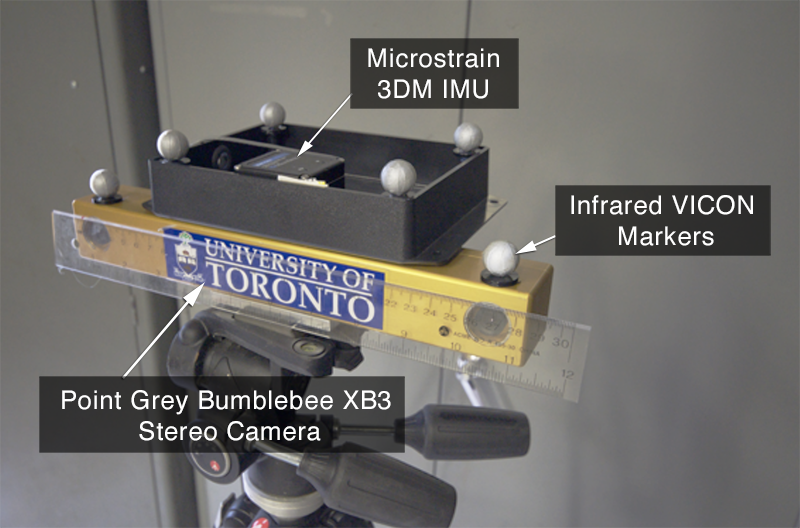
\includegraphics[width=0.45\textwidth]{figs/sensorhead}
    \caption{The sensor head used in our experiments. The IMU measures translational and rotational velocities, while the stereo camera measures the positions of point landmarks. In our experiments, we artificially blinded the stereo camera by using measurements from the left camera only.}
    \label{fig:sensorhead}
\end{figure}

\begin{figure}
    \centering
    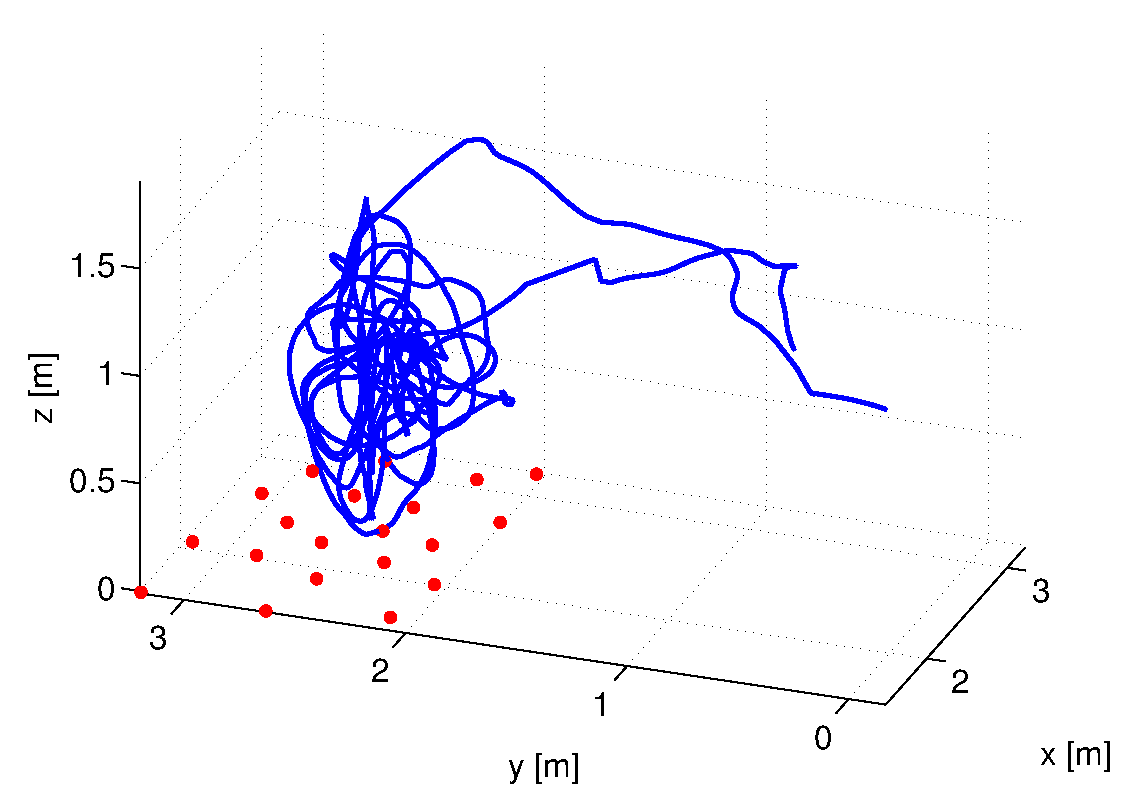
\includegraphics[width=0.48\textwidth]{figs/trajectory_groundtruth}
    \caption{Vicon ground truth for sensor head motion (blue) and landmark positions (red) in the ``Starry Night'' dataset.}
    \label{fig:trajectory_groundtruth}
\end{figure}

Things quickly got out of hand when Matlab achieved sentience. 
We were forced to abandon our lab and have been surviving in the harsh environment of the MarsDome for weeks.
If this ever gets published, please send help!





%%%%%%%%%%%%%%%%%%%%%%%%%%%%%%%%%%%%%%%%%%%%%%%%%%%%%%%%%%%%%%%%%%%%%%%%%%%%%%%%
\section{CONCLUSIONS} \label{sec:conclusions}

%%%%%%%%%%%%%%%%%%%%%%%%%%%%%%%%%%%%%%%%%%%%%%%%%%%%%%%%%%%%%%%%%%%%%%%%%%%%%%%%
%%%%%%%%%%%%%%%%%%%%%%%%%%%%%%%%%%%%%%%%%%%%%%%%%%%%%%%%%%%%%%%%%%%%%%%%%%%%%%%%
%\section*{ACKNOWLEDGMENT}
%\vspace{8pt}
%%%%%%%%%%%%%%%%%%%%%%%%%%%%%%%%%%%%%%%%%%%%%%%%%%%%%%%%%%%%%%%%%%%%%%%%%%%%%%%%

\def\url#1{} % Get rid of url in citations -- also had to modify IEEEtran.bst
\bibliographystyle{IEEEtran}
\bibliography{project_bib.bib}

\end{document}
